% Created 2019-08-22 jeu. 11:06
% Intended LaTeX compiler: pdflatex
\documentclass[t]{clean-beamer}
\usepackage[utf8]{inputenc}
\usepackage[T1]{fontenc}
\usepackage{graphicx}
\usepackage{grffile}
\usepackage{longtable}
\usepackage{wrapfig}
\usepackage{rotating}
\usepackage[normalem]{ulem}
\usepackage{amsmath}
\usepackage{textcomp}
\usepackage{amssymb}
\usepackage{capt-of}
\usepackage{hyperref}
\usepackage[most]{tcolorbox}
\usepackage{siunitx}
\AtBeginSection[]{
\begin{frame}<beamer>{Table of Contents}
\tableofcontents[currentsection, hideothersubsections, sectionstyle=show/shaded]
\end{frame}
}
\usetheme{default}
\author{Dehaeze Thomas}
\date{07-11-2019}
\title{Complementary Filters Shaping\newline Using \(\mathcal{H}_\infty\) Synthesis}
\subtitle{ICCMA 2019}
\hypersetup{
 pdfauthor={Dehaeze Thomas},
 pdftitle={Complementary Filters Shaping\newline Using \(\mathcal{H}_\infty\) Synthesis},
 pdfkeywords={complementary filters, h-infinity, sensor fusion},
 pdfsubject={Complementary Filters Shaping Using H-Infinity Synthesis. Presentation at ICCMA 2019.},
 pdfcreator={Emacs 26.2 (Org mode 9.2.5)},
 pdflang={English}}
\begin{document}

\maketitle
\begin{frame}{Outline}
\tableofcontents
\end{frame}


\section{Introduction}
\label{sec:org4eff5bb}
\label{sec:introduction}

\begin{frame}[label={sec:org6dbc4f9}]{Introduction}
High bandwidth
\begin{itemize}
\item need of Sensor at low frequency + sensor at high frequency
\item need of merging the two
\item complementary filters
\item design of those filters using \(\mathcal{H}_\infty\)
\end{itemize}
\end{frame}

\section{Complementary Filters Requirements}
\label{sec:org49f4bb1}
\label{sec:requirements}
\begin{frame}[label={sec:orgd4e76ba}]{Sensor Fusion Architecture}
\label{sec:sensor_fusion}

\begin{figure}[htbp]
\centering
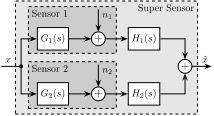
\includegraphics[scale=1]{figs/fusion_super_sensor.pdf}
\caption{\label{fig:fusion_super_sensor}
Sensor fusion architecture}
\end{figure}

\begin{equation}
\label{eq:comp_filter_estimate}
  \hat{x} = \left(G_1 H_1 + G_2 H_2\right) x + H_1 n_1 + H_2 n_2
\end{equation}

\begin{equation}
\label{eq:comp_filter}
  H_1(s) + H_2(s) = 1
\end{equation}
\end{frame}

\begin{frame}[label={sec:org1234068}]{Noise Sensor Filtering}
\label{sec:noise_filtering}

Perfect Sensor Dynamics:
\begin{equation}
\label{eq:perfect_dynamics}
  G_1(s) = G_2(s) = 1
\end{equation}

Super Sensor Estimation:
\begin{equation}
\label{eq:estimate_perfect_dyn}
  \hat{x} = x + H_1 n_1 + H_2 n_2
\end{equation}

Noise in the Super Sensor:
\begin{equation}
\label{eq:noise_filtering_psd}
  \Phi_{\delta x} = \left|H_1\right|^2 \Phi_{n_1} + \left|H_2\right|^2 \Phi_{n_2}
\end{equation}

Usually, the two sensors have high noise levels over distinct frequency regions.
In order to lower the noise of the super sensor, the value of the norm \(|H_1|\) has to be lowered when \(\Phi_{n_1}\) is larger than \(\Phi_{n_2}\) and that of \(|H_2|\) lowered when \(\Phi_{n_2}\) is larger than \(\Phi_{n_1}\).
\end{frame}

\begin{frame}[label={sec:org9e26d3e}]{Robustness of the Fusion}
\label{sec:fusion_robustness}

\begin{figure}[htbp]
\centering
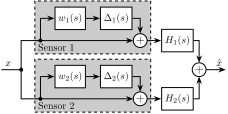
\includegraphics[scale=1]{figs/sensor_fusion_dynamic_uncertainty.pdf}
\caption{\label{fig:sensor_fusion_dynamic_uncertainty}
Sensor fusion architecture with sensor dynamics uncertainty}
\end{figure}

\begin{equation}
\label{eq:super_sensor_dyn_uncertainty}
  \frac{\hat{x}}{x} = 1 + w_1(s) H_1(s) \Delta_1(s) + w_2(s) H_2(s) \Delta_2(s)
\end{equation}

\begin{equation}
\label{eq:max_uncertainty_super_sensor}
  \begin{aligned}
    & \left|w_1 H_1 \Delta_1\right| + \left|w_2 H_2 \Delta_2\right| \le \epsilon \quad \forall\omega,\ \forall \Delta_1, \forall \Delta_2\\
    \Leftrightarrow & \left|w_1 H_1\right| + \left|w_2 H_2\right| \le \epsilon \quad \forall\omega
  \end{aligned}
\end{equation}
\end{frame}

\section{Complementary Filters Shaping using \(\mathcal{H}_\infty\) Synthesis}
\label{sec:org727d73b}
\label{sec:hinf_method}
\begin{frame}[label={sec:org3adefc5}]{Shaping of Complementary Filters using \(\mathcal{H}_\infty\) synthesis}
\label{sec:hinf_synthesis}

Synthesis Objective:
\begin{subequations}
\label{eq:comp_filter_problem_form}
  \begin{align}
  & H_1(s) + H_2(s) = 1 \label{eq:hinf_cond_complementarity} \\
  & |H_1(j\omega)| \le \frac{1}{|W_1(j\omega)|} \quad \forall\omega \label{eq:hinf_cond_h1} \\
  & |H_2(j\omega)| \le \frac{1}{|W_2(j\omega)|} \quad \forall\omega \label{eq:hinf_cond_h2}
  \end{align}
\end{subequations}

\begin{figure}[htbp]
\centering
\includegraphics[scale=1]{figs/h_infinity_robust_fusion.pdf}
\caption{\label{fig:h_infinity_robust_fusion}
Architecture used for \(\mathcal{H}_\infty\) synthesis of complementary filters}
\end{figure}

\begin{equation}
\label{eq:hinf_syn_obj}
  \left\|\begin{matrix} \left[1 - H_2(s)\right] W_1(s) \\ H_2(s) W_2(s) \end{matrix}\right\|_\infty \le 1
\end{equation}

\begin{equation}
\label{eq:definition_H1}
  H_1(s) \triangleq 1 - H_2(s)
\end{equation}
\end{frame}

\begin{frame}[label={sec:org90726d8}]{Weighting Functions Design}
\label{sec:hinf_weighting_func}
\begin{equation}
\label{eq:weight_formula}
  W(s) = \left( \frac{
           \hfill{} \frac{1}{\omega_0} \sqrt{\frac{1 - \left(\frac{G_0}{G_c}\right)^{\frac{2}{n}}}{1 - \left(\frac{G_c}{G_\infty}\right)^{\frac{2}{n}}}} s + \left(\frac{G_0}{G_c}\right)^{\frac{1}{n}}
         }{
           \left(\frac{1}{G_\infty}\right)^{\frac{1}{n}} \frac{1}{\omega_0} \sqrt{\frac{1 - \left(\frac{G_0}{G_c}\right)^{\frac{2}{n}}}{1 - \left(\frac{G_c}{G_\infty}\right)^{\frac{2}{n}}}} s + \left(\frac{1}{G_c}\right)^{\frac{1}{n}}
         }\right)^n
\end{equation}

\begin{figure}[htbp]
\centering
\includegraphics[scale=1]{figs/weight_formula.pdf}
\caption{\label{fig:weight_formula}
Magnitude of a weighting function generated using the formula}
\end{figure}
\end{frame}

\begin{frame}[label={sec:orgbb615dc}]{Validation of the proposed synthesis method}
\label{sec:hinf_example}
\begin{figure}[htbp]
\centering
\includegraphics[scale=1]{figs/hinf_synthesis_results.pdf}
\caption{\label{fig:hinf_synthesis_results}
Frequency response of the weighting functions and complementary filters obtained using \(\mathcal{H}_\infty\) synthesis}
\end{figure}
\end{frame}

\begin{frame}[label={sec:org1e9511a}]{Synthesis of Three Complementary Filters}
\label{sec:hinf_three_comp_filters}
\begin{figure}[htbp]
\centering
\includegraphics[scale=1]{figs/comp_filter_three_hinf.pdf}
\caption{\label{fig:comp_filter_three_hinf}
Architecture for \(\mathcal{H}_\infty\) synthesis of three complementary filters}
\end{figure}

\begin{figure}[htbp]
\centering
\includegraphics[scale=1]{figs/hinf_three_synthesis_results.pdf}
\caption{\label{fig:hinf_three_synthesis_results}
Frequency response of the weighting functions and three complementary filters obtained using \(\mathcal{H}_\infty\) synthesis}
\end{figure}
\end{frame}

\section{Application: Design of Complementary Filters used in the Active Vibration Isolation System at the LIGO}
\label{sec:org282c8fb}
\label{sec:application_ligo}
\begin{frame}[label={sec:org17c24af}]{Application}
Several complementary filters are used in the active isolation system at the LIGO \cite{hua05_low_ligo,hua04_polyp_fir_compl_filter_contr_system}.
The requirements on those filters are very tight and thus their design is complex.
The approach used in \cite{hua05_low_ligo} for their design is to write the synthesis of complementary FIR filters as a convex optimization problem.
The obtained FIR filters are compliant with the requirements. However they are of very high order so their implementation is quite complex.

The effectiveness of the proposed method is demonstrated by designing complementary filters with the same requirements as the one described in \cite{hua05_low_ligo}.
\end{frame}

\begin{frame}[label={sec:org1f8bc6e}]{Complementary Filters Specifications}
\label{sec:ligo_specifications}
\begin{itemize}
\item From \(0\) to \(\SI{0.008}{Hz}\), the magnitude of the filter's transfer function should be less or equal to \(8 \times 10^{-4}\)
\item Between \(\SI{0.008}{Hz}\) to \(\SI{0.04}{Hz}\), the filter should attenuate the input signal proportional to frequency cubed
\item Between \(\SI{0.04}{Hz}\) to \(\SI{0.1}{Hz}\), the magnitude of the transfer function should be less than \(3\)
\item Above \(\SI{0.1}{Hz}\), the magnitude of the complementary filter should be less than \(0.045\)
\end{itemize}

\begin{figure}[htbp]
\centering
\includegraphics[scale=1]{figs/ligo_weights.pdf}
\caption{\label{fig:ligo_weights}
Specifications and weighting functions magnitude used for \(\mathcal{H}_\infty\) synthesis}
\end{figure}
\end{frame}

\begin{frame}[label={sec:org305a6e1}]{Weighting Functions Design}
\label{sec:ligo_weights}

\begin{figure}[htbp]
\centering
\includegraphics[scale=1]{figs/ligo_weights.pdf}
\caption{\label{fig:ligo_weights}
Specifications and weighting functions magnitude used for \(\mathcal{H}_\infty\) synthesis}
\end{figure}
\end{frame}

\begin{frame}[label={sec:org1aa43d2}]{\(\mathcal{H}_\infty\) Synthesis}
\label{sec:ligo_results}

\begin{figure}[htbp]
\centering
\includegraphics[scale=1]{figs/comp_fir_ligo_hinf.pdf}
\caption{\label{fig:comp_fir_ligo_hinf}
Comparison of the FIR filters (solid) designed in \cite{hua05_low_ligo} with the filters obtained with \(\mathcal{H}_\infty\) synthesis (dashed)}
\end{figure}
\end{frame}

\section{Conclusion}
\label{sec:org425430e}
\label{sec:conclusion}
\begin{frame}[label={sec:org3cfbc70}]{Conclusion}
This paper has shown how complementary filters can be used to combine multiple sensors in order to obtain a super sensor.
Typical specification on the super sensor noise and on the robustness of the sensor fusion has been shown to be linked to the norm of the complementary filters.
Therefore, a synthesis method that permits the shaping of the complementary filters norms has been proposed and has been successfully applied for the design of complex filters.
Future work will aim at further developing this synthesis method for the robust and optimal synthesis of complementary filters used in sensor fusion.
\end{frame}
\section{Bibliography}
\label{sec:org404b871}
\begin{frame}[label={sec:org03eccb0}]{Bibliography}
\bibliographystyle{unsrt}
\bibliography{ref}
\end{frame}
\end{document}